\section*{1. Zeitplanung}
\label{zeitplanung}
    \begin{itemize}
        \item Analysephase (5 Stunden)
            \begin{itemize}
                \item Ist-Analyse (2 Stunden)
                \item Ermitteln des Soll-Zustands, Verfassung eines Lasten- und Pflichtenhefts (3 Stunden)
            \end{itemize}
        \item Frontendentwicklung (32 Stunden):
            \begin{itemize}
                \item UX Design (3 Stunden)
                \item Login-Seite (2 Stunden)
                \item Hauptoberfläche (7 Stunden)
                \item Tag-Funktion/Suchfunktion (8 Stunden)
                \item Notizeditor (8 Stunden)
                \item Testphase (4 Stunden)
            \end{itemize}
        \item Backendentwicklung (35 Stunden)
            \begin{itemize}
                \item Datenbank-Design (2 Stunden)
                \item Datenbank-Verbindung (2 Stunden)
                \item Entwicklung der API:
                \begin{itemize}
                    \item Login-Funktion (6 Stunden)
                    \item Synchronisierung zwischen Usern (8 Stunden)
                    \item Speichern und auslesen von Tags (6 Stunden)
                    \item Speichern und auslesen von Notizen (6 Stunden)
                    \item Testphase (5 Stunden)
                \end{itemize}
            \end{itemize}
        \item Dokumentation (8 Stunden)
    \end{itemize}

\section*{2. Kanban-Board}
\label{kanban}
    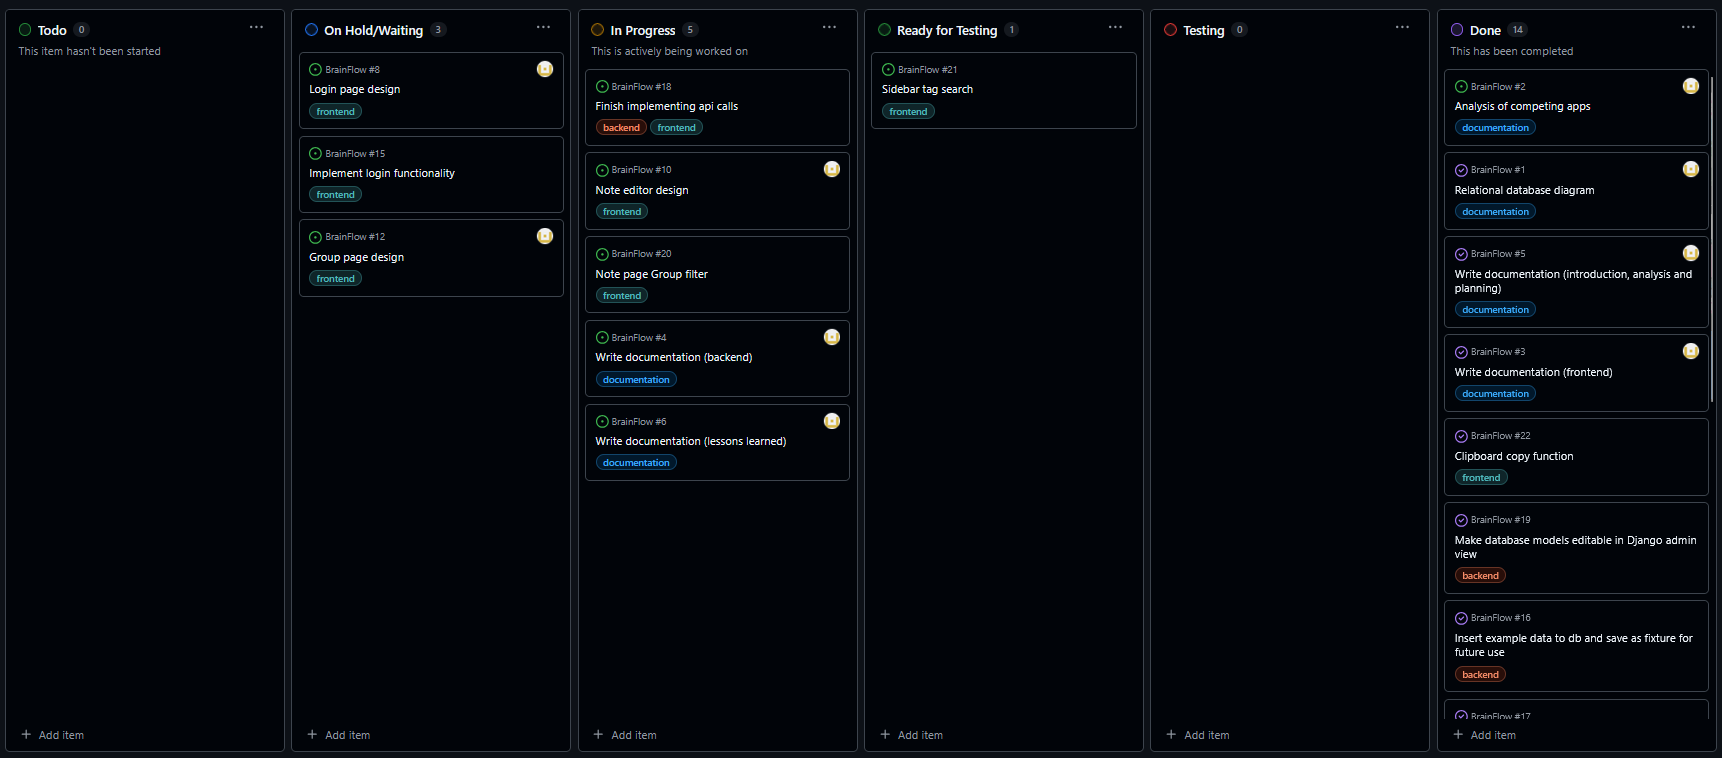
\includegraphics[angle=90, origin=c, width=0.75\linewidth]{kanban.png}

\section*{3.1 Use Case Diagramm}
\label{usecase}
    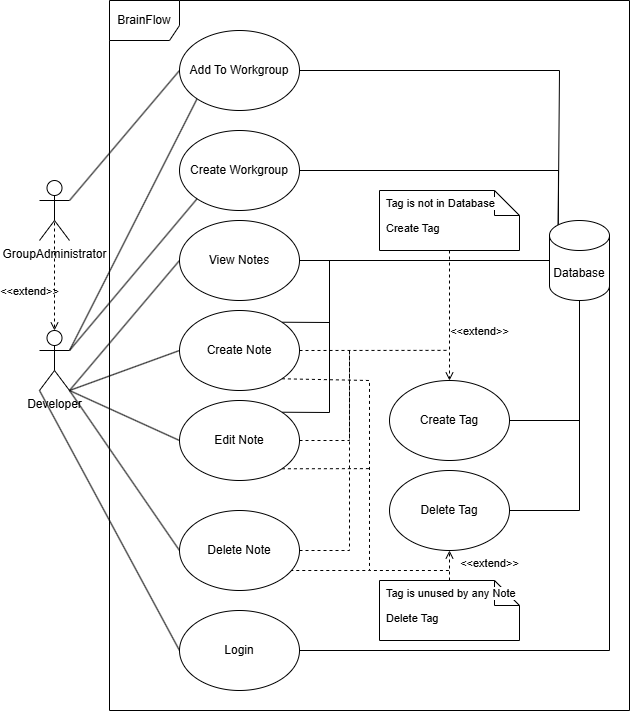
\includegraphics[width=0.65\textwidth]{usecase_full.png}

\section*{3.2 Mockup}
\label{mockup}
    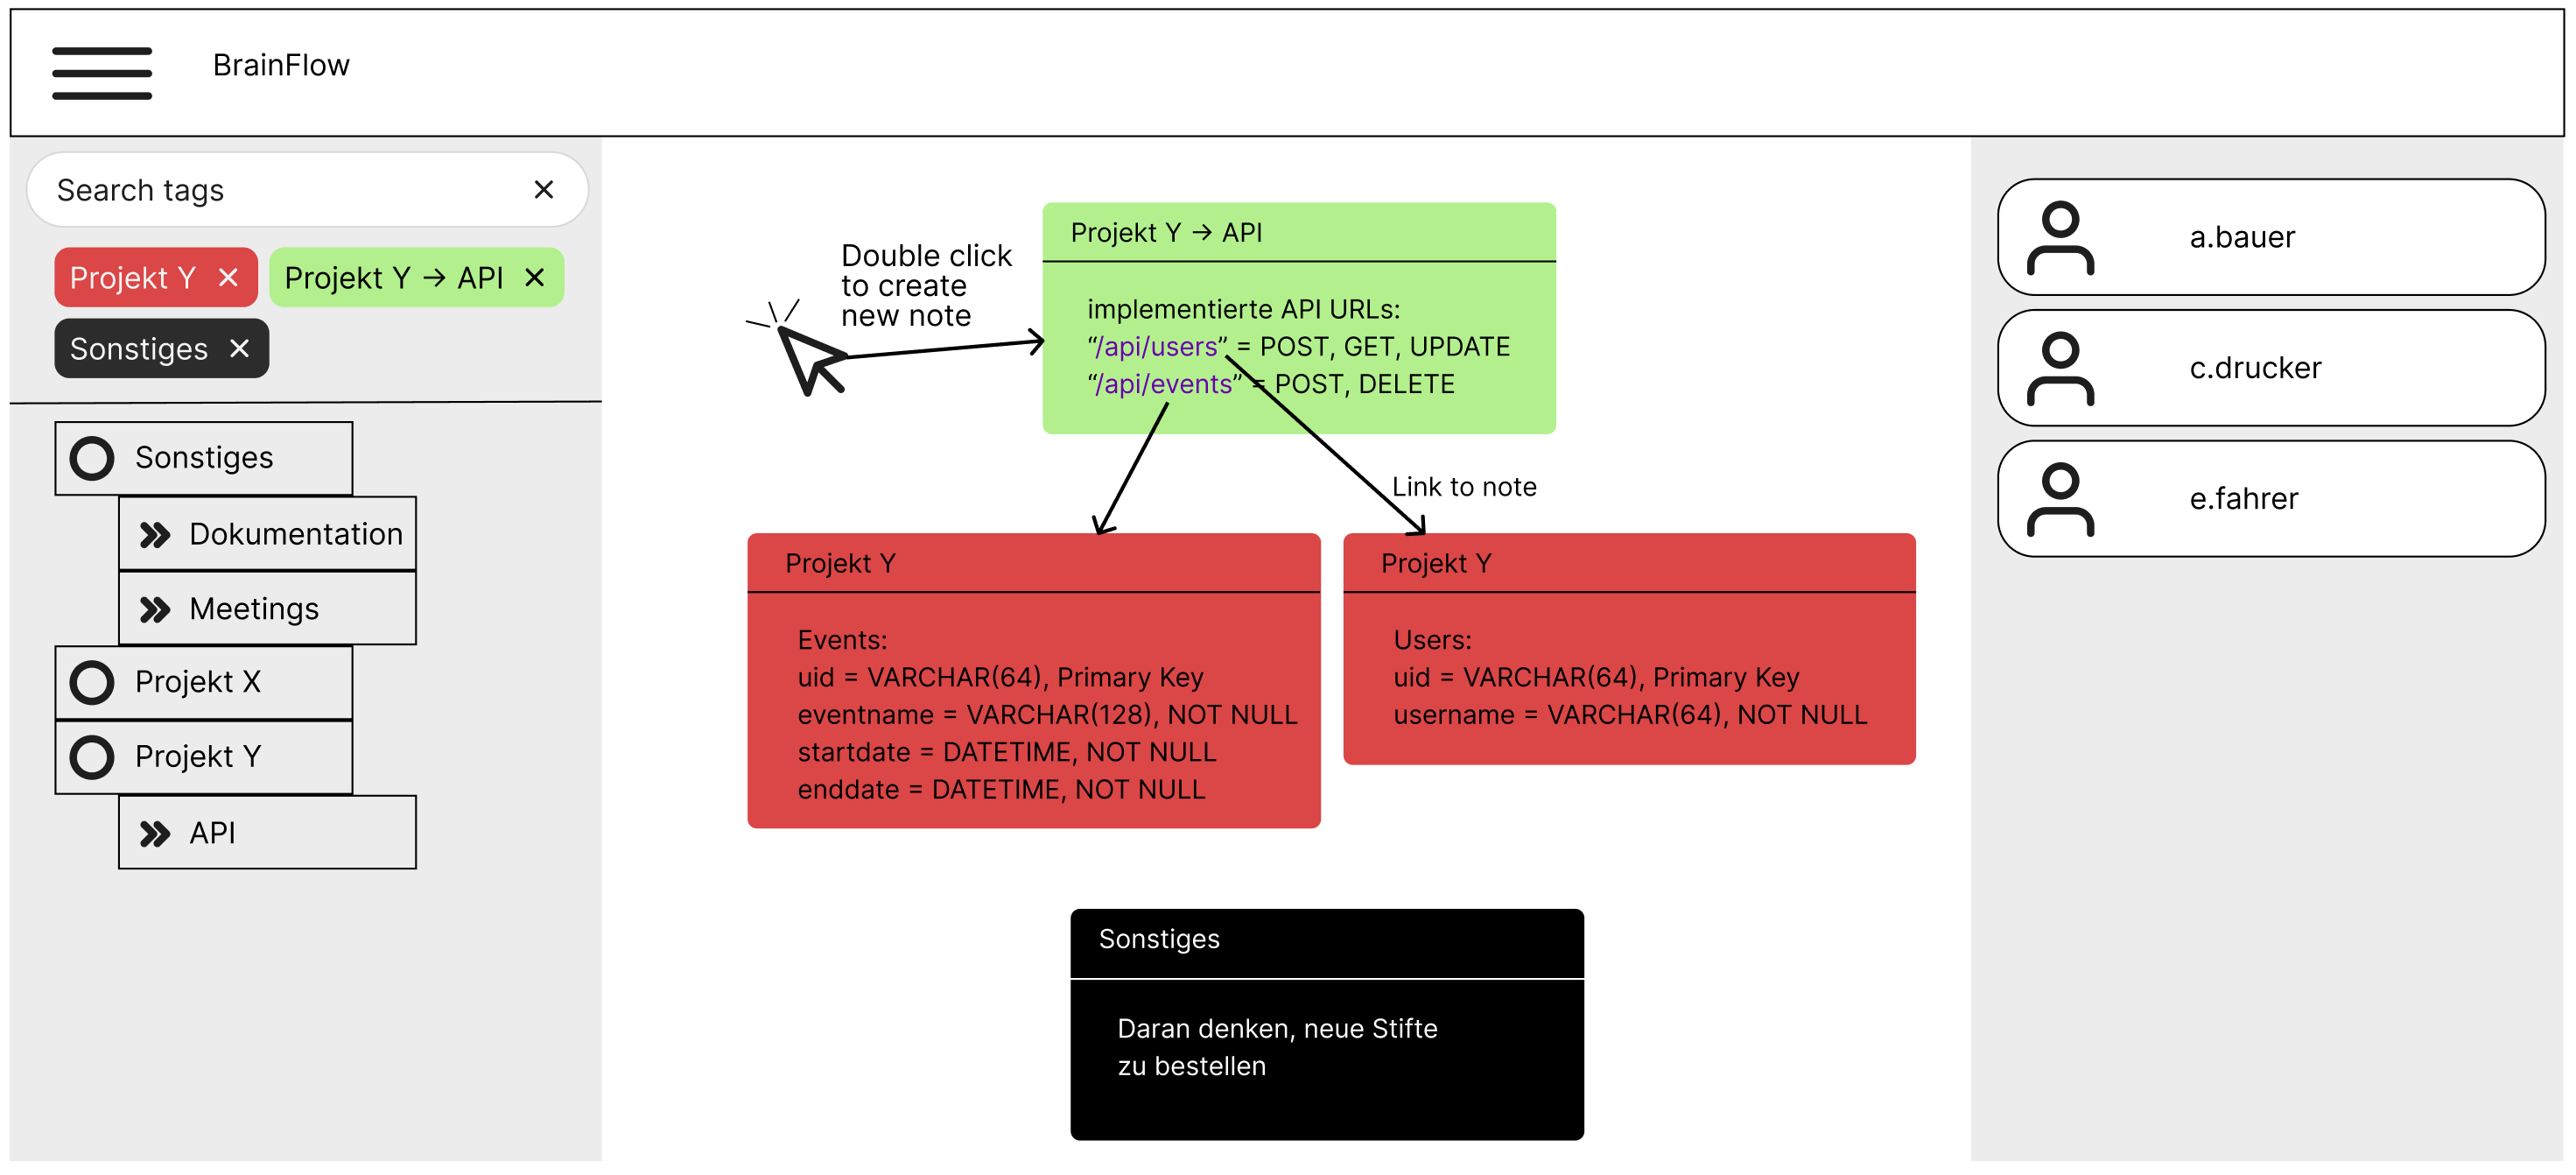
\includegraphics[width=\textwidth]{mockup_full.png}

\section*{4.1 Notizen-Seite}
\label{ui}
    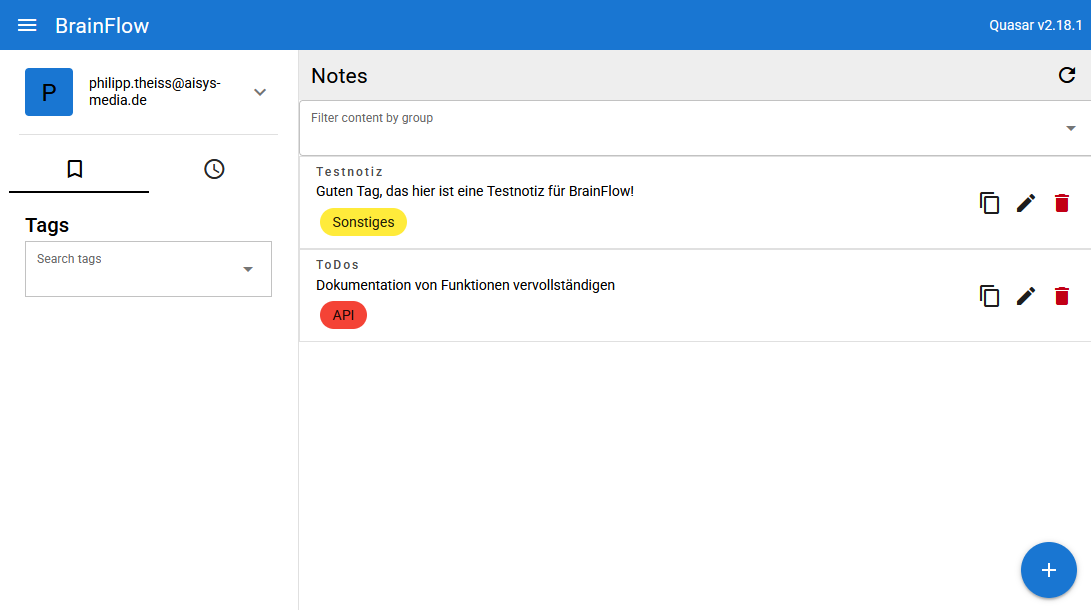
\includegraphics[width=0.8\textwidth]{ui.png}

\section*{4.2 Notizen Code}
\label{notes}
    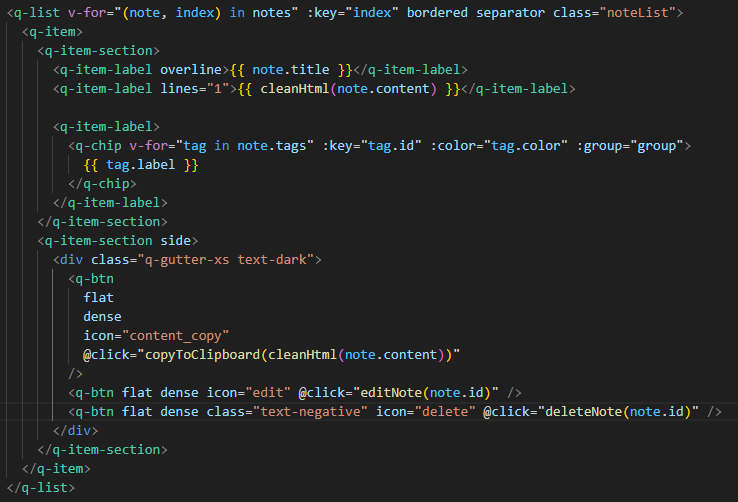
\includegraphics[width=\textwidth]{notes.png}

\section*{4.3 Pinia State}
\label{pinia}
    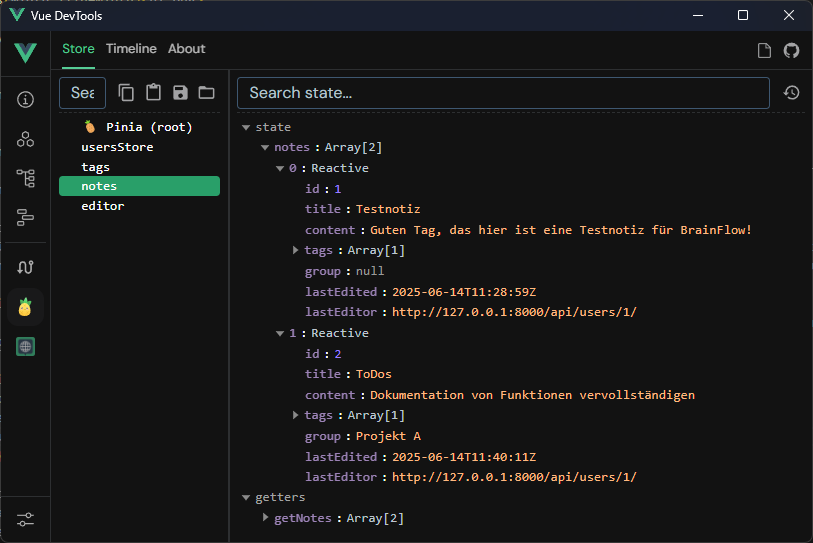
\includegraphics[width=\textwidth]{pinia.png}

\section*{4.4 Axios API}
\label{api}
    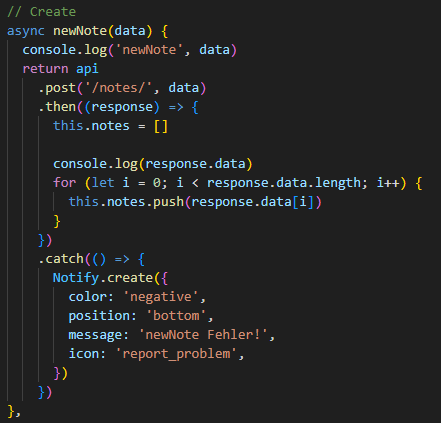
\includegraphics[width=0.5\textwidth]{api.png}

\section*{5.1 ER-Modell}
\label{erm}
    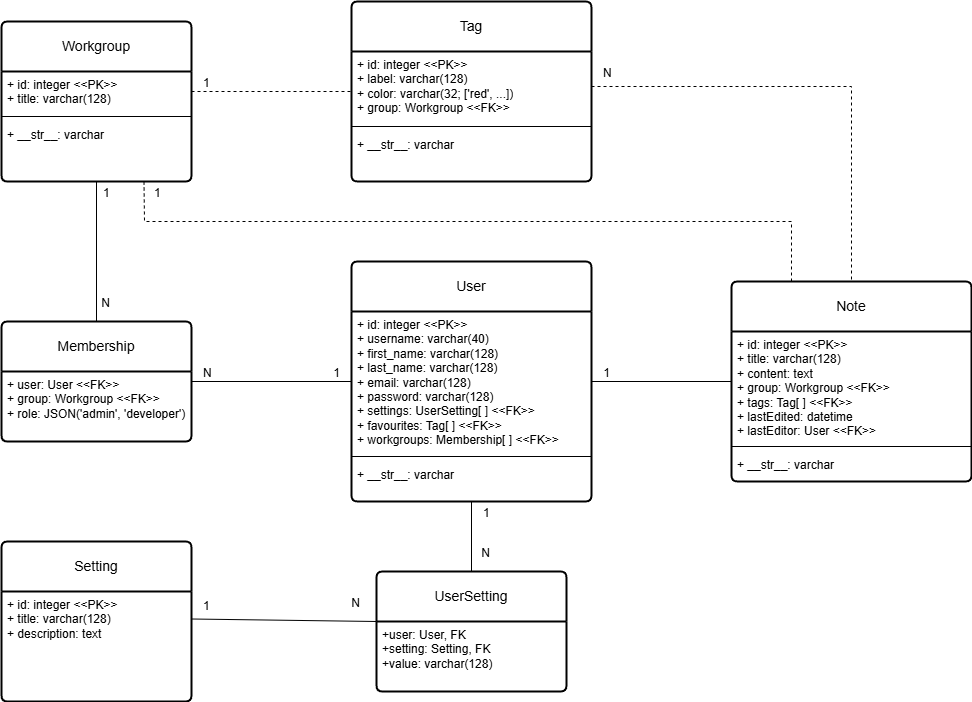
\includegraphics[width=\textwidth]{ER_Model.png}

\section*{5.2 Admin Menü}
\label{admin}
    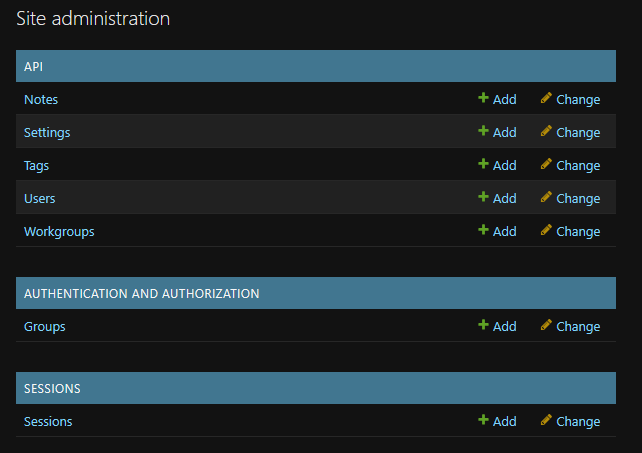
\includegraphics[width=\textwidth]{admin1.png}

\section*{5.3 Admin Menü M-zu-N}
\label{admin2}
    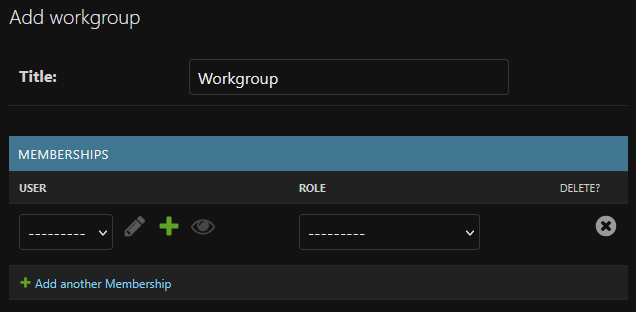
\includegraphics[width=\textwidth]{admin2.png}